\subsection{Is there tilt, and can an HMM see it?}
\begin{figure}[t]
\centering
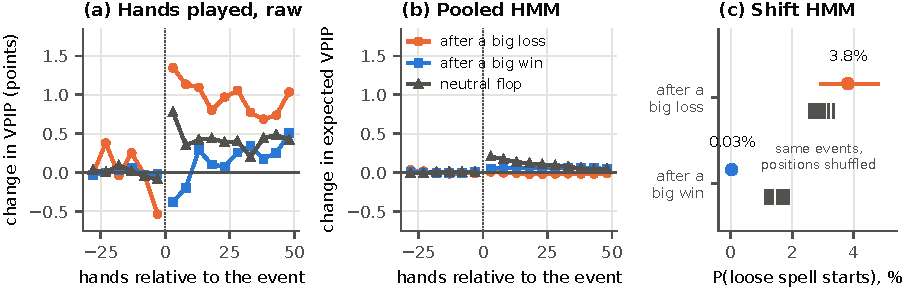
\includegraphics[width=\linewidth]{../figures/fig_tilt.pdf}
\caption{Held-out data. (a) Change in the share of hands played (VPIP) around big losses, big wins and neutral flops, relative to the player's own 30 hands before; 5-hand bins. (b) The same for the pooled HMM's posterior-expected VPIP, on the same scale. (c) Shift HMM with input-dependent transitions: probability that a loose spell starts at the first hand after an event, with 95\% bootstrap intervals; grey ticks are 20 fits with the event positions shuffled within sessions.}
\label{fig:tilt}
\end{figure}
\textbf{The raw effect is real and small.} Held-out sessions contain 13{,}957 big losses by 1{,}420 players with clean windows. In the 30 hands after a big loss players enter 1.07 points more pots than in the 30 hands before (base 22.9\%); after a big win the change is $+0.02$ and after a neutral flop $+0.46$ (Figure~\ref{fig:tilt}a). The neutral control shows that part of the rise is mechanical: the ``before'' window is required to contain no big pot, which selects quiet hands. Net of controls the loss effect is $\mathbf{+1.04}$ \textbf{points against wins} (95\% interval 0.78 to 1.31) and $+0.60$ against neutral flops (0.40 to 0.83): part loosening after losses, part tightening after wins, the ``trying to break even'' of Thaler and Johnson \cite{thaler1990} and the direction Smith et al.\ \cite{smith2009} found at high stakes. The effect is still visible 50 hands later, is larger at the lowest stake ($+1.41$ against $+0.88$) and for low-volume players, and does not depend on the threshold (Table~\ref{tab:sub}). Players also quit within 30 hands more often after a big loss (9.1\%) than after a big win (7.2\%). Across the 613 players with five or more big losses, effects vary by about 1.3 points (standard deviation) beyond sampling noise.

\textbf{The pooled HMM cannot see it.} The same event study on the pooled model's filtered posteriors is flat (Figure~\ref{fig:tilt}b); the loss-minus-win difference in posterior-expected VPIP is $-0.07$ points. This follows from assumption (v): the states are four fixed styles 3 to 18 VPIP points apart that last hundreds of hands, and a one-point shift is not a move between them. The input-output extension does not help: it raises training log-likelihood by 10.6 nats, where inputs shuffled within sessions raise it by 5.6 on average, and on held-out data it is 12 to 31 nats \emph{worse} than the plain HMM (Table~\ref{tab:io}).

\textbf{Each player as their own baseline.} If the states are busy describing who the player is, take that job away. One emission table per player with \emph{no} hidden state reaches $-0.699$ per decision on test data, against $-0.751$ for the pooled four-state HMM and $-0.736$ for eight states: knowing who is playing is worth more than any number of pooled states. A free second mode per player adds at most 0.0014 and over-fits unless a strong prior keeps the modes close (Table~\ref{tab:personal}).

\textbf{The shift HMM finds loose spells, and losses start them.} With the emissions of Eq.~(\ref{eq:shift}), two states and three symbols, EM finds a ``loose'' state with $\theta=(0.50,0.30)$ for calling and raising: odds of calling up 65\% and of raising up 35\% relative to folding, which moves an average player from playing 25.9\% of their decisions to 32.3\%. The state holds 6.9\% of test hands, starts about once in 5{,}000 hands and lasts about 300. It adds 0.0005 nats per decision on test data, 200 times less than the pooled model's hidden states, and a no-switching version with tight, normal and loose \emph{sessions} adds slightly more (0.0007): variation within a player is small and mostly between sessions. Unlike the pooled model's, this state's posterior moves the right way, rising 0.49 points more after a big loss than after a big win (0.26 to 0.72). With input-dependent transitions we obtain the estimate the proposal asked for (Figure~\ref{fig:tilt}c). The probability of entering the loose state is 0.012\% at an ordinary hand, \textbf{3.8\%} (2.9 to 4.8) at the first hand after a big loss, and 0.03\% (0.005 to 0.15) after a big win. Shuffled event positions give 2.9\% (at most 3.3\% in 20 draws) and 1.5\%, far above the ordinary rate because loose play causes big pots, so events cluster in sessions that contain spells. Against that benchmark a real loss is 1.3 times as likely to start a spell and a real win almost never does. The input does not improve held-out likelihood beyond the shuffled versions (33 nats against 30): this is an estimate of a transition probability, not a better predictor.

\textbf{Answer to question 2.} Yes in direction, no in the form we proposed. The tilt state is rare (a few percent of big losses), long (hundreds of hands, not the 20 to 50 we guessed) and accounts for at most a quarter of the average shift ($3.8\%\times6.4$ points); the rest is a diffuse change that no discrete state captures.

\textbf{Alternative explanations.} (1) \emph{Selection}: players in a loose spell are more likely to play big pots at all; the controls and the shuffled inputs share this. (2) \emph{Stack size}: a loss leaves a shorter stack at that table, which changes correct play; but for players on three or more tables most later hands are at other tables with unchanged stacks, and the effect is the same ($+1.01$). (3) \emph{Rational adjustment}: a big pot reveals information about opponents; we cannot separate deliberate adjustment from emotion, so ``tilt'' names the behavioural pattern only. (4) \emph{Who stays}: players who quit after a loss are not in the after-window, so we may under-estimate.

\subsection{Ablations and a negative control}
\label{sec:ablations}
\textbf{Context} is the most valuable modeling choice: on a common task (predicting fold, check/call or raise one step ahead; Table~\ref{tab:abl}) it improves held-out log-likelihood by 0.10 to 0.12 nats per decision, more than the hidden states do. Our stated reason for it was wrong, though: an HMM without context does not spend its states on the position cycle (decoded state and position are unrelated in every variant, Cram\'er's $V<0.01$), because sticky states cannot follow something that changes every hand. Context matters for fit, not for what the states mean. \textbf{Alphabet}: on that task the eight-symbol model predicts slightly \emph{worse} than the three-symbol one ($-0.615$ against $-0.609$); its extra symbols go to raise-size habits.

\textbf{Sequence length} (Figure~\ref{fig:ablation}a). Cutting training sessions into pieces of 5 hands lowers held-out log-likelihood by 0.016 and the learned self-transition from 0.998 to 0.970; beyond about 100 hands nothing is lost. Sequences must be long enough to accumulate evidence about a style, not to watch it change.

\textbf{Pooled or per player} (Figure~\ref{fig:ablation}b,c). With shared emissions, a transition matrix per player improves log-likelihood on later sessions from $-0.711$ to $-0.698$, best with the weakest shrinkage: it acts as a memory of the player's style. A fully personal four-state HMM matches the pooled one after about 500 of the player's own hands and beats it for 81\% of players after 1{,}000. The pooled model is right for a new player and wrong for a known one.

\textbf{Negative control} (Table~\ref{tab:pluribus}). Pluribus plays one fixed strategy, so a sound method should find no modes in its 10{,}000 hands. It finds none: a personal HMM with $K=2,3,4$ has lower cross-validated log-likelihood than $K=1$. The sobering side: the same test finds none in five of the six human professionals who played it, nor in 72\% of 40 PartyPoker players with as many hands.
